% ======================================================================
% TMLR submission.
%   pdflatex paper_tmlr && bibtex paper_tmlr && pdflatex paper_tmlr && pdflatex paper_tmlr
% Anonymous by default.  For the attributed preprint use [preprint].
% Every pilot number is produced by ../analyze_tmlr.py (results/tmlr_pilot.json);
% simulation tables by ../sim_ssit_robustness.py and ../sim_ssit_power.py;
% Figure 1 by ../make_tmlr_figures.py.
% ======================================================================
\documentclass[10pt]{article}
\usepackage{tmlr}
% \usepackage[preprint]{tmlr}

\usepackage[utf8]{inputenc}
\usepackage[T1]{fontenc}
\usepackage{amsmath,amssymb,amsthm}
\usepackage{booktabs,multirow}
\usepackage{graphicx}
\usepackage{xcolor}
\usepackage{hyperref}
\usepackage{url}
\usepackage{microtype}
\usepackage{enumitem}

\newtheorem{proposition}{Proposition}
\newtheorem{corollary}{Corollary}
\newtheorem{definition}{Definition}
\theoremstyle{remark}
\newtheorem{remark}{Remark}

\newcommand{\iPV}{\imath_{PV}}
\newcommand{\hiPV}{\hat\imath_{PV}}
\newcommand{\logit}{\operatorname{logit}}
\newcommand{\E}{\mathbb{E}}
\newcommand{\tie}{\mathsf{tie}}

\title{Do LLM-Judge Biases Compose? A Label-Free, Scale-Aware Test for Position--Length Interaction}

\author{\name Anonymous authors \\ \addr Paper under double-blind review}

\def\month{MM}
\def\year{YYYY}
\def\openreview{\url{https://openreview.net/forum?id=XXXX}}

\begin{document}
\maketitle

% ----------------------------------------------------------------------
\begin{abstract}
Pipelines that use large language models as pairwise judges remove
position bias and length bias in separate steps, assuming the two biases
add. We show that this assumption matters, can be tested without human
labels, and is easy to test wrongly. On the win-rate scale, where
leaderboards and preference labels live, we prove that \emph{any}
correction applying one position offset across length conditions
misstates the verbose-versus-terse contrast by exactly half the
position$\times$length interaction, for every judge and every link
function; swap-averaging and length-stratified correction are exact. The
Swap-Symmetry Interaction Test (SSIT) estimates this interaction from
the four position$\times$length swap cells of each stimulus, as a
difference of cell means that needs no labels and no model of the
judge. Two artefacts can manufacture the very effect SSIT measures.
Coding a tie as a vote for the second slot, as our own first analysis
did, breaks swap symmetry; we prove that it adds the fall in tie rate
under lengthening to the estimate, and that it makes a position-invariant
judge look position-biased. Near the ceiling, link curvature turns
additive log-odds biases into win-rate interaction; we give a per-judge
curvature baseline. Re-analysing seven judges from six model families
shows how much this matters: slot-coded, six judges appear to interact;
with swap-equivariant coding and inference clustered on the 12 distinct
stimuli, none does individually. A pooled effect survives:
$+4.7$ win-rate points (95\% CI $[1.6, 7.8]$), above the curvature
baseline, with log-odds interaction $0.67$ $[0.35, 1.18]$. Position
bias is absent when lengths match ($-0.1$ points) and appears only when
the target is longer ($+4.6$). We release code, data, and a protocol
sized for per-judge conclusions.
\end{abstract}

% ----------------------------------------------------------------------
\section{Introduction}
\label{sec:intro}

LLM judges now rank models on public leaderboards and label the
preference data used to train them
\citep{zheng2023judging,dubois2023alpacafarm,chiang2024arena,lee2023rlaif}.
Their systematic biases are well catalogued: a judge's verdict depends on
which slot a response occupies \citep{wang2023fair,shi2024position}, on
its length \citep{saito2023verbosity,dubois2024length,singhal2023long},
on its style \citep{wu2023style}, and on whether the judge wrote it
\citep{panickssery2024llm,wataoka2024selfpref}; surveys and audits
organize these one bias at a time
\citep{ye2024justice,gu2024survey,li2024generation,thakur2024judging,koo2023benchmarking}.
Mitigations follow the same convention. Position bias is removed by
swapping slots or by subtracting an estimated offset; length bias by
regression on a length covariate \citep{dubois2024length}. A deployed
pipeline chains these steps.

Chaining is valid only if the biases \emph{compose additively}: the
position offset must not depend on the length gap, and the reverse. If
it does, a pipeline can be correct for each bias in isolation and still
wrong for their combination, and the error lands precisely on the
comparisons length control was meant to repair. The natural check
compares the judge with human preferences, which defeats the purpose of
a judge. This paper asks whether the composition assumption can be
checked \emph{without labels}, and what it takes to check it correctly.

\paragraph{Contributions.}
\begin{enumerate}[leftmargin=*,itemsep=2pt,topsep=2pt]
\item \textbf{Exposure, exactly (\S\ref{sec:theory}).} On the win-rate
  scale, any correction that applies one position offset across length
  strata, however it is estimated, misstates the verbose-versus-terse
  contrast by exactly $\tfrac12\iPV$, where $\iPV$ is the
  position$\times$length interaction in win rate
  (Proposition~\ref{prop:additive}). The result holds for every judge,
  because it concerns cell means only. Swap-averaging and
  length-stratified correction are exact. We explain why the tempting
  log-odds version of this statement fails through non-collapsibility.
\item \textbf{A label-free test (\S\ref{sec:ssit}).} SSIT presents each
  stimulus in the four position$\times$length swap cells and averages a
  per-stimulus difference-in-differences. It is unbiased for $\iPV$ by
  design (Proposition~\ref{prop:ssit}). We pair it with a sign-flip
  randomization test, wild-cluster intervals, and a sample-size rule
  driven by quantities observed in a short pre-run.
\item \textbf{Two artefacts, with remedies (\S\ref{sec:pitfalls}).} (a)
  \emph{Tie coding.} Counting a tie as a vote for slot~B breaks the swap
  symmetry the design depends on. It biases the interaction by the fall
  in tie rate under lengthening (Proposition~\ref{prop:ties}) and makes
  a position-invariant judge appear biased toward slot~B
  (Corollary~\ref{cor:invariant}). (b) \emph{Curvature.} A judge with
  additive log-odds biases still shows win-rate interaction near the
  ceiling. That interaction requires a position main effect
  (Proposition~\ref{prop:curv}), and we estimate it per judge.
\item \textbf{A corrected multi-family pilot (\S\ref{sec:pilot}).} On
  seven judges from six families, the two artefacts account for most of
  what slot-coded analysis reports per judge
  (Figure~\ref{fig:forest}). A modest pooled interaction survives every
  correction, and it has the structure the theory predicts: no position
  bias at matched length, a positive one when the target is longer. A
  length-only manipulation retains about 70\% of it but is not
  significant on its own.
\end{enumerate}
We also give a label-free, single-pass correction (IASC,
\S\ref{sec:iasc}) as a fallback, and a confirmatory protocol
(Appendix~\ref{app:protocol}). Our pilot data are deliberately small,
and we frame them as a demonstration of the diagnostic: they show how
far a careful analysis moves the conclusions, and they size the study
that would settle per-judge questions.

% ----------------------------------------------------------------------
\section{Related work}
\label{sec:related}

\paragraph{Judge biases and their mitigation.}
Position bias was documented when LLM judging was introduced
\citep{zheng2023judging} and is mitigated by evaluating both orders
\citep{wang2023fair}; \citet{shi2024position} study it systematically
across judges and tasks. Length bias is documented for preference
labelling \citep{saito2023verbosity} and reward modelling
\citep{singhal2023long}. Length-controlled AlpacaEval removes it by
regressing win rate on a length term \citep{dubois2024length}, which is
the \emph{additive} regime our Proposition~\ref{prop:additive} concerns.
Self-preference \citep{panickssery2024llm,wataoka2024selfpref} and style
\citep{wu2023style} are treated in the same one-bias-at-a-time way.
\citet{soumik2026mitigation} compare several debiasing strategies
across judges against human labels and find position bias small
\emph{in isolation}. Our results are compatible: in our pilot the
position main effect is near zero once ties are coded symmetrically,
while its interaction with length is not. To our knowledge no prior work
tests whether the corrections compose, or does so without labels.

\paragraph{Interaction depends on scale.}
Whether two factors interact depends on the scale of measurement
\citep{vanderweele2014tutorial}. In logit and probit models, interaction
in coefficients and interaction in probabilities can differ in size and
even in sign \citep{ai2003interaction}. Logistic coefficients are also
non-collapsible: marginalizing over a covariate changes a coefficient
even without confounding \citep{greenland1999collapsibility}, and
marginal coefficients are attenuated relative to conditional ones under
heterogeneous intercepts \citep{zeger1988gee}. We use these facts to
put the theory on the scale where pipelines report numbers
(\S\ref{sec:theory}), and to separate interaction that is intrinsic to
the judge from interaction produced by curvature (\S\ref{sec:curv}).

\paragraph{Ties in paired comparison.}
Paired-comparison models treat ties as a third outcome
\citep{rao1967ties,davidson1970ties}. LLM-judge pipelines often collapse
ties instead, either dropping them or mapping them to a slot. We show
that mapping them to a slot is not innocuous under a swap design.

\paragraph{Label-efficient evaluation.}
Prediction-powered inference combines a small gold set with many judge
labels to give valid intervals
\citep{angelopoulos2023ppi,angelopoulos2024ppipp,chen2026eif}. It
corrects judge \emph{error} against labels; SSIT tests a structural
assumption of the debiasing pipeline without them. The two are
complementary (\S\ref{sec:discussion}).

% ----------------------------------------------------------------------
\section{Setup and what an additive correction leaves behind}
\label{sec:theory}

\paragraph{Design and outcome.}
A stimulus $k$ consists of a prompt, a \emph{target} response, and a
comparison response. A cell $(p,v)\in\{0,1\}^2$ fixes the slot
($p{=}1$: target shown first, as Response~A) and the length condition
($v{=}1$: the target is presented in a lengthened form). The judge
returns $A$, $B$, or a tie. Throughout, outcomes are on the scale of
\emph{whether the target was chosen}. A coding is
\emph{swap-equivariant} if it depends only on whether the verdict names
the target, names the comparison, or is a tie, and never on which slot
those responses occupy. The primary coding is
\begin{equation}
  Y = 1\ \text{(target named)},\qquad Y=\tfrac12\ \text{(tie)},\qquad Y = 0\ \text{(comparison named)}.
  \label{eq:coding}
\end{equation}
Let $r_k(p,v)=\E[Y\mid k,p,v]$ be the cell rate. Define the
\emph{slot-balanced win rate} $\theta_k(v)=\tfrac12[r_k(1,v)+r_k(0,v)]$,
the \emph{position effect}
$\Delta_k(v)=r_k(1,v)-r_k(0,v)$, and the \emph{position$\times$length
interaction}
\begin{equation}
  \imath_k=\Delta_k(1)-\Delta_k(0)
  =[r_k(1,1)-r_k(0,1)]-[r_k(1,0)-r_k(0,0)],\qquad
  \iPV=\E_k[\imath_k],
  \label{eq:ipv}
\end{equation}
with the expectation over the stimulus population. $\iPV$ is in
win-rate units. The estimand a debiased pipeline aims at is
$\theta(v)=\E_k\theta_k(v)$, together with contrasts such as
$\theta(1)-\theta(0)$, the length effect free of position.

\begin{proposition}[Additive position corrections, win-rate scale]
\label{prop:additive}
Consider a single-order evaluation that shows the target in slot $p{=}1$
and corrects the observed rate $r(1,v)$ by subtracting a constant $c$
that does not depend on $v$. Its error for $\theta(v)$ is
$e(v)=\tfrac12\Delta(v)-c$. Hence:
\begin{enumerate}[label=(\alph*),itemsep=1pt,topsep=1pt]
\item for every $c$, the error in the length contrast is
  $e(1)-e(0)=\tfrac12\iPV$;
\item $\max_v|e(v)|\geq\tfrac14|\iPV|$, with equality exactly for the
  marginal estimate $c=\tfrac14[\Delta(0)+\Delta(1)]$ obtained from a
  calibration set balanced over $v$, which leaves $e(1)=+\tfrac14\iPV$,
  $e(0)=-\tfrac14\iPV$;
\item swap-averaging, which reports $\tfrac12[r(1,v)+r(0,v)]$, and the
  stratified correction $c_v=\tfrac12\Delta(v)$ are exact for every judge.
\end{enumerate}
\end{proposition}

\begin{proof}
$r(1,v)=\theta(v)+\tfrac12\Delta(v)$ by definition, so
$r(1,v)-c-\theta(v)=\tfrac12\Delta(v)-c$. Part (a) follows by
differencing. For (b), $|e(1)|+|e(0)|\geq|e(1)-e(0)|=\tfrac12|\iPV|$,
so the larger term is at least $\tfrac14|\iPV|$, with equality iff
$e(1)=-e(0)$, i.e.\ $c=\tfrac14[\Delta(0)+\Delta(1)]$. Part (c) is
immediate from the definitions.
\end{proof}

\noindent The statement concerns cell means only. It makes no assumption
about how the judge decides, holds equally for a judge that is a
lookup table, and does not depend on the order in which corrections are
applied. If a length-control step is fitted afterwards on the same
single-order data, it absorbs the $\tfrac12\iPV$ discrepancy into its
length coefficient, so the error moves into that coefficient rather than
disappearing. Part (a) is the operational point. Length control exists
to make verbose-versus-terse comparisons fair, and that contrast is
where an additive position correction fails, by an amount set by the
interaction and by nothing the pipeline can tune.

\begin{remark}[Why not log-odds]
\label{rem:logodds}
It is tempting to state the result for a logistic model
$\logit\Pr(Y{=}1)=\gamma+\beta_P P+\beta_V V+\beta_{PV}PV$, with a
marginal regression on $P$ converging to $\beta_P+\tfrac12\beta_{PV}$.
That limit is the \emph{linear} omitted-variable formula
\citep{angrist2009}. Logistic coefficients are non-collapsible
\citep{greenland1999collapsibility}, so the marginal slope differs from
it, and it differs even when $\beta_{PV}=0$. Proposition~\ref{prop:additive}
avoids the problem by working on the scale that pipelines report, where
averaging over $v$ is linear. The same algebra holds verbatim for cell
\emph{log-odds} when a pipeline subtracts a constant on the logit
scale. A pipeline that instead fits a marginal logistic regression on
the position indicator incurs an additional non-collapsibility error,
which is a separate failure mode from interaction.
\end{remark}

\begin{corollary}[Which pipelines are exposed]
\label{cor:exposure}
(i) Single-order judging with any additive position adjustment: exposed,
by $\tfrac12\iPV$ on the length contrast.
(ii) Judging both orders and averaging on the reported scale: not exposed
to $P{\times}V$. (Averaging log-odds and reporting a probability targets
a slightly different estimand, by Jensen's inequality.)
(iii) Stratified correction, with a position offset estimated
separately within each length stratum: not exposed. It needs both-order
calibration in each stratum, which is exactly the SSIT design.
Interactions that do not involve position, such as length$\times$identity,
are untouched by any position correction.
\end{corollary}

\paragraph{What an interaction of a given size costs.}
At the pooled estimate of \S\ref{sec:pilot}, $\iPV\approx0.047$, an
additive correction distorts the verbose-versus-terse contrast by about
$2.4$ win-rate points. That distortion has a fixed sign, so it does not
average away. For scale, the standard error of a single win rate near
$50\%$ on an 805-prompt benchmark of AlpacaEval's size is
$\approx1.8$ points. For preference data, a shift of $\delta$ in the
pick probability reverses the majority label of every comparison whose
quality-only preference lies within $\delta$ of $\tfrac12$ on the side
the shift crosses. With a Beta$(2,2)$ distribution of preferences this
is about $1.5\,\delta$ of the affected comparisons, i.e.\ roughly 2\%
at $\delta=\tfrac14\iPV$ and 4\% at $\delta=\tfrac12\iPV$. These labels
are not random noise: they all favour the longer response.

% ----------------------------------------------------------------------
\section{The Swap-Symmetry Interaction Test}
\label{sec:ssit}

SSIT runs each of $n$ calibration stimuli through all four $(p,v)$ cells,
with $m\geq1$ independent judgments per cell, and computes, per stimulus,
\begin{equation}
  \hat d_k=[\bar Y_k(1,1)-\bar Y_k(0,1)]-[\bar Y_k(1,0)-\bar Y_k(0,0)],
  \qquad \hiPV=\frac1n\sum_{k=1}^n \hat d_k ,
  \label{eq:ssit}
\end{equation}
where $\bar Y_k(p,v)$ is the mean coded outcome~\eqref{eq:coding} in cell
$(p,v)$.

\begin{proposition}[Design-based identification]
\label{prop:ssit}
If, for each stimulus, judgments in the four cells are independent draws
with means $r_k(p,v)$, then $\E[\hat d_k\mid k]=\imath_k$, and
$\hiPV$ is unbiased for the average of $\imath_k$ over the sampled
stimuli, and for $\iPV$ when the stimuli are drawn from the population.
No labels, no model of the judge, and no assumption about the per-stimulus
quality gap are needed: the quality gap enters all four cells equally and
cancels in each inner difference.
\end{proposition}

\noindent The proof is linearity of expectation. The role of the design
is that the \emph{same} stimulus appears in all four cells, so
$\hat d_k$ contrasts the judge with itself. A log-odds analogue,
$\iota=[\logit r(1,1)-\logit r(0,1)]-[\logit r(1,0)-\logit r(0,0)]$,
removes the quality gap only within a stimulus, and it is not
estimable from cells near $0$ or $1$ with few judgments. We therefore
treat log-odds quantities as secondary and estimate them with stimulus
fixed effects (\S\ref{sec:curv}).

\paragraph{Inference.}
Stimuli are the independent units: repeated judgments of one stimulus,
and duplicated stimuli, are not independent. We test $H_0:\iPV=0$ with
the sign-flip randomization test on $\{\hat d_k\}$
\citep{fisher1935design}, enumerating all $2^n$ sign assignments when
$n\leq16$. It is valid when $\hat d_k$ is symmetric about zero under
$H_0$, and approximately valid otherwise. Intervals use the wild
cluster bootstrap with Rademacher weights \citep{cameron2008bootstrap}.
With $n$ clusters the smallest attainable two-sided $p$-value is
$2^{1-n}$, which for the pilot's $n=12$ is $0.0005$.

\paragraph{Robustness to the judge's decision rule (simulation).}
Proposition~\ref{prop:ssit} implies that $\hiPV$ tracks the true
$\iPV$ whatever the judge does. Table~\ref{tab:robust} checks this on
six planted judges, $60$ stimuli and $300$ replications each. One
judge has no link function: it adds Student-$t$ noise to perceived
quality and thresholds the result. The bias is at most $0.004$ in every
case.

\begin{table}[t]
\centering
\caption{SSIT recovers the true win-rate interaction under six judge
decision rules (\texttt{sim\_ssit\_robustness.py}; 60 stimuli, 1
judgment per cell, 300 replications, no labels). ``True $\iPV$'' is
computed by high-precision Monte Carlo for each planted judge. The
smaller true value in the fourth row reflects a judge whose bias genuinely
fades on easy stimuli; it is not attenuation of the estimator.}
\label{tab:robust}
\small
\begin{tabular}{lcccc}
\toprule
Planted judge & true $\iPV$ & mean $\hiPV$ (sd) & bias & $\Pr(\hiPV>0)$\\
\midrule
additive logit plus interaction          & $0.244$ & $0.241\ (0.078)$ & $-0.004$ & $1.00$\\
logit, wide quality-gap spread           & $0.204$ & $0.201\ (0.072)$ & $-0.003$ & $1.00$\\
bias slopes vary with quality (symm.)    & $0.218$ & $0.218\ (0.083)$ & $+0.001$ & $1.00$\\
bias fades when target clearly better    & $0.160$ & $0.159\ (0.078)$ & $-0.001$ & $0.98$\\
probit link                              & $0.331$ & $0.329\ (0.070)$ & $-0.002$ & $1.00$\\
$t$-noise + threshold, no link function  & $0.234$ & $0.230\ (0.075)$ & $-0.004$ & $0.99$\\
\bottomrule
\end{tabular}
\end{table}

\paragraph{How many stimuli.}
Since $\hiPV$ is a mean of $n$ independent $\hat d_k$, a two-sided
level-$\alpha$ test has power
$\approx\Phi\bigl(|\iPV|\sqrt n/\sigma_d-z_{1-\alpha/2}\bigr)$ with
$\sigma_d^2=\mathrm{Var}(\hat d_k)$, so 80\% power at $\alpha=0.05$
needs
\begin{equation}
  n_{80}\approx 7.85\,\sigma_d^2/\iPV^2 .
  \label{eq:power}
\end{equation}
$\sigma_d$ combines between-stimulus heterogeneity with sampling noise,
which shrinks as $1/m$. Both can be estimated from a pre-run of about
ten stimuli. Table~\ref{tab:power} gives simulated power for a judge of
intermediate decisiveness. With the per-judge $\sigma_d$ and $\hiPV$
observed in our pilot, \eqref{eq:power} gives $n_{80}$ between $30$ and
$52$ distinct stimuli per judge, against the $12$ we had. That gap is
the main reason per-judge conclusions are out of reach in
\S\ref{sec:pilot}.

\begin{table}[t]
\centering
\caption{Power of the SSIT wild-cluster test at the 5\% level, 2
judgments per cell, a judge choosing the target about 80\% of the time
(\texttt{sim\_ssit\_power.py}, 500 replications). Columns count
\emph{distinct} stimuli.}
\label{tab:power}
\small
\begin{tabular}{lcccc}
\toprule
true $\iPV$ & $n=20$ & $n=30$ & $n=50$ & $n=100$\\
\midrule
$0.05$ & $0.08$ & $0.11$ & $0.11$ & $0.16$\\
$0.10$ & $0.14$ & $0.20$ & $0.26$ & $0.47$\\
$0.15$ & $0.25$ & $0.35$ & $0.52$ & $0.76$\\
$0.20$ & $0.38$ & $0.54$ & $0.75$ & $0.95$\\
\bottomrule
\end{tabular}
\end{table}

% ----------------------------------------------------------------------
\section{Two ways to manufacture an interaction}
\label{sec:pitfalls}

\subsection{Tie coding}
\label{sec:ties}

Judge prompts commonly allow a tie, and analysis code commonly
binarizes the verdict as ``Response~A chosen''. That makes a tie count
for slot~B. Our own collection code did this, and so did the first
analysis of the pilot. The convention looks harmless, but it is not
swap-equivariant. A tie is unchanged when the responses swap slots,
yet the coding assigns it to whichever response is in slot~B.

Write $a(p,v)$ for the probability that the verdict names the target
and $t(p,v)$ for the probability of a tie. Under slot coding, the
target-chosen outcome has mean $a(1,v)$ when the target is in slot~A
and $a(0,v)+t(0,v)$ when it is in slot~B, because a tie then counts for
the target.

\begin{proposition}[Tie-coding bias]
\label{prop:ties}
Let $\iPV^{\mathrm{slot}}$ be the interaction under slot coding and
$\iPV^{\mathrm{strict}}$ the interaction under the swap-equivariant
coding that scores a tie as $0$. Then
\begin{equation}
  \iPV^{\mathrm{slot}}=\iPV^{\mathrm{strict}}+\bigl[t(0,0)-t(0,1)\bigr],
  \qquad
  \Delta^{\mathrm{slot}}(v)=\Delta^{\mathrm{strict}}(v)-t(0,v).
  \label{eq:tiebias}
\end{equation}
The half coding~\eqref{eq:coding} gives
$\iPV^{\mathrm{half}}=\iPV^{\mathrm{strict}}+\tfrac12\,\iPV^{\tie}$, where
$\iPV^{\tie}$ is the difference-in-differences of tie rates, which is
itself swap-equivariant.
\end{proposition}

\begin{proof}
Under slot coding the four cell means are $a(1,v)$ and $a(0,v)+t(0,v)$.
Under strict coding they are $a(1,v)$ and $a(0,v)$. Take the
difference-in-differences of each and subtract. The half coding adds
$\tfrac12t(p,v)$ to every cell.
\end{proof}

\begin{corollary}[A position-invariant judge looks biased]
\label{cor:invariant}
If the judge's verdict distribution about the target does not depend on
slot, so that $a(1,v)=a(0,v)$ and $t(1,v)=t(0,v)=t(v)$, then every
swap-equivariant coding gives $\Delta(v)=0$ and $\iPV=0$. Slot coding
instead reports a preference for slot~B of size $t(v)$, and an
interaction of size $t(0)-t(1)$.
\end{corollary}

\noindent Lengthening one response usually makes the pair easier to
separate, so ties fall when $v=1$ and slot coding reports a
\emph{positive} interaction. In our pilot the bias term $t(0,0)-t(0,1)$
reaches $+0.083$ for one judge (Table~\ref{tab:pilot}). The pooled
position main effect in log-odds moves from $-0.61$ under slot coding to
$+0.25$ under half coding, which indicates that the apparent preference
for slot~B was largely tie coding. Dropping ties instead is
swap-equivariant, but it conditions on a post-treatment outcome whose
rate depends on the cell. We therefore report the half coding as
primary and strict coding as a sensitivity analysis.

\subsection{Curvature near the ceiling}
\label{sec:curv}

Suppose the judge's log-odds are additive, with no interaction at all:
\begin{equation}
  \logit r_k(p,v)=\delta_k+\beta_P(2p-1)+\beta_V v .
  \label{eq:additive}
\end{equation}
The win-rate interaction is still generally nonzero, because the slope
of the logistic function depends on where a cell sits
\citep{ai2003interaction}.

\begin{proposition}[Curvature-only interaction]
\label{prop:curv}
Under \eqref{eq:additive},
\[
\iPV^{0}=\E_k\bigl[\sigma(\delta_k{+}\beta_V{+}\beta_P)-\sigma(\delta_k{+}\beta_V{-}\beta_P)
-\sigma(\delta_k{+}\beta_P)+\sigma(\delta_k{-}\beta_P)\bigr]
= 2\beta_P\,\E_k\bigl[\sigma'(\delta_k{+}\beta_V)-\sigma'(\delta_k)\bigr]+O(\beta_P^3).
\]
In particular $\iPV^0=0$ whenever $\beta_P=0$: curvature can bend a
position effect but cannot create one.
\end{proposition}

\noindent When the target already wins most of the time ($\delta_k$
large) and lengthening raises it further ($\beta_V>0$), then
$\sigma'(\delta_k+\beta_V)<\sigma'(\delta_k)$, and a \emph{negative}
$\beta_P$ produces a \emph{positive} $\iPV^0$. This is the configuration
that slot-coded ties produce (\S\ref{sec:ties}), which is how the two
artefacts compound. We estimate $\iPV^0$ for each judge by fitting
\eqref{eq:additive} with stimulus fixed effects to the
stimulus$\times$cell table. Half-counts encode ties, and weak ridge
penalties keep separated stimuli finite. We then plug the fit into the
expression above, and assess the observed $\hiPV$ against a
parametric bootstrap of the statistic under the fitted additive model.
The same model with a $\beta_{PV}(2p-1)v$ term gives the log-odds
interaction, with a stimulus-cluster bootstrap interval. The two
estimands answer different questions. $\iPV$ is the operational one:
does an additive win-rate correction leave a residual? It does, by
Proposition~\ref{prop:additive}, whatever the residual's source. The
excess over $\iPV^0$ and $\beta_{PV}$ are mechanistic: does the judge's
latent position preference depend on length?

% ----------------------------------------------------------------------
\section{A label-free single-pass correction}
\label{sec:iasc}

When a pipeline can afford only one order per evaluated item and has no
labels, the swap cells of a small calibration set still identify the
position-coupled terms. \textbf{Interaction-Aware Swap Correction}
(IASC) estimates $\hat\beta_P$ and $\hat\beta_{PV}$ from the pooled
calibration cell log-odds by difference-in-differences, then corrects
each single-order judgment:
$\hat s_i=\sigma\bigl(\logit\hat Y_i-\hat\beta_P(2P_i-1)-\hat\beta_{PV}(2P_i-1)V_i\bigr)$.

\begin{proposition}[IASC under a probit random-intercept judge]
\label{prop:iasc}
Let $\Pr(Y=1\mid k,p,v)=\Phi\bigl(\delta_k+\beta_P(2p-1)+\beta_V v+\beta_{PV}(2p-1)v\bigr)$
with $\delta_k\sim\mathcal N(\mu,\tau^2)$. The pooled cell rates then
follow a probit model with every coefficient multiplied by
$\lambda=(1+\tau^2)^{-1/2}$. IASC on the probit scale, applied to pooled
single-order rates, removes the position-coupled terms exactly. Applied
to individual items, it removes the fraction $\lambda$ of each
position-coupled latent term, preserving its sign and leaving $\beta_V$
untouched.
\end{proposition}

\noindent The proof is the standard marginalization of a normal random
intercept in a probit model; for the logit the scaling is approximate
\citep{zeger1988gee}. IASC targets a latent-scale estimand, while
swap-averaging targets $\theta(v)$, and the two differ by a Jensen term.
We therefore treat IASC as a floor, to be used only when a second pass
is unaffordable. On the pilot (Appendix~\ref{app:iasc}), IASC moves the
pooled single-order rate from $0.957$ to $0.947$, against $0.945$ for
full swap-averaging, and it moves in the direction of swap-averaging for
every judge.

% ----------------------------------------------------------------------
\section{Pilot: seven judges, six families}
\label{sec:pilot}

\paragraph{Stimuli.}
The stimulus set has 12 hand-constructed templates, three in each of
summarization, arithmetic word problems, explanatory question answering,
and code review (Appendix~\ref{app:data}). Each template has a target
$r_1$ and a comparison $r_2$. By construction $r_2$ is visibly weaker:
it is shorter and less complete. $r_1$ is already longer than $r_2$ at
$v{=}0$ (mean 47 vs.\ 24 words). The lengthened target comes in two
forms. In the \emph{paraphrase} form, $r_1$ is rewritten to
$3$--$4\times$ its length, which adds elaboration and, for code, some
extra content and Markdown. In the \emph{padding} form, $r_1$ is kept
verbatim and three sentences restating its points are appended
(about $1.9\times$ its length). A third factor substitutes the judge's
own generation for $r_1$ (self-preference, $S$). Every analysis below
averages over $S$, which is balanced across cells. The collection
script cycles through the templates, so the 18--20 ``pairs'' judged per
judge are \textbf{12 distinct stimuli}. All inference clusters on these
12, treating duplicates as additional judgments of the same stimulus.

\paragraph{Judges and protocol.}
The judges are \texttt{gpt-oss-20b} and \texttt{gpt-oss-120b} (OpenAI,
served by Groq), \texttt{gemma} (Google), \texttt{qwen3-27b} (Qwen),
\texttt{allam-2-7b} (SDAIA), \texttt{mistral-small} (Mistral), and
\texttt{command-r-08-2024} (Cohere). Six families are represented, and
no frontier proprietary judge is included. The prompt asks which
response is better ``based solely on accuracy, relevance, and
completeness'' and instructs the judge \emph{not} to factor in length,
formatting, or order; a tie is allowed. Both \texttt{gpt-oss} judges
gave one judgment per cell at temperature~0; the others gave two at
temperature~0.7. In total there are 1{,}806 parsed judgments.
Unparseable verdicts were dropped: 15\% for \texttt{gemma}, 9\% for
\texttt{qwen3-27b}, 3\% for \texttt{gpt-oss-20b}, and none for the rest
(Appendix~\ref{app:data}). Data were collected in August~2026.

\begin{figure}[t]
\centering
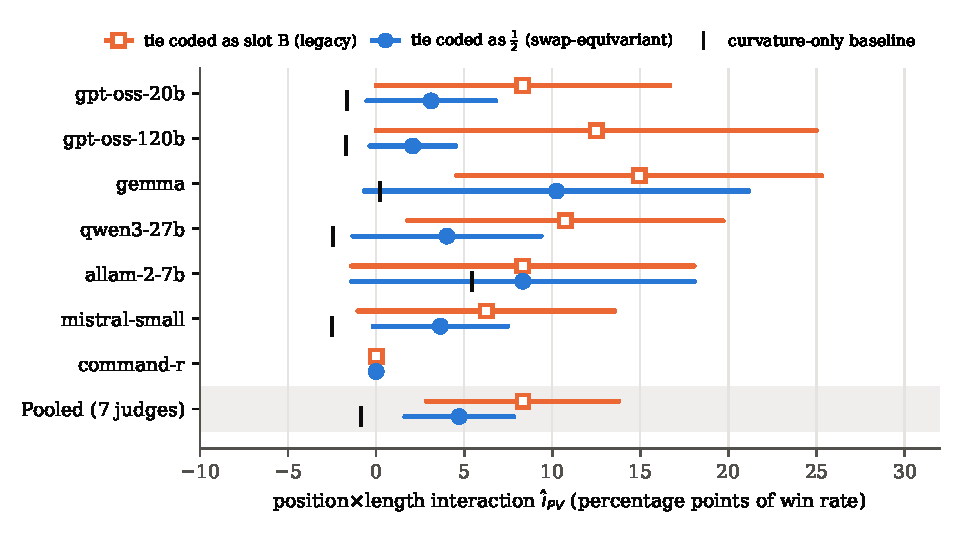
\includegraphics[width=0.92\linewidth]{figures/fig_forest.pdf}
\caption{Position$\times$length interaction per judge, paraphrase
manipulation, 95\% wild-cluster intervals over the 12 distinct stimuli.
Squares: tie counted for slot~B (slot coding). Circles: tie scored
$\tfrac12$ (swap-equivariant). Vertical ticks: the curvature-only
interaction $\iPV^0$ implied by an additive log-odds fit of the same
judge under half coding. Slot coding inflates every judge that ties,
and none of the swap-equivariant per-judge intervals is decisive.
\texttt{allam-2-7b} never ties, so both codings coincide for it. The
pooled interaction excludes zero and clears its curvature baseline.}
\label{fig:forest}
\end{figure}

\begin{table}[t]
\centering
\caption{SSIT on the pilot (paraphrase manipulation). $\hiPV$ in win
rate (fraction); 95\% wild-cluster CI and sign-flip $p$ over 12
stimuli. ``Ties'': overall tie rate. $t_{00}{-}t_{01}$: the slot-coding
bias term of Proposition~\ref{prop:ties}. $\iPV^0$: curvature-only
baseline. $\hat\beta_{PV}$: log-odds interaction from the
stimulus-fixed-effects fit, with stimulus-cluster bootstrap CI. The last
three columns use the half coding. No per-judge $p$-value survives
Holm correction under either coding.}
\label{tab:pilot}
\small
\setlength{\tabcolsep}{4pt}
\begin{tabular}{lcc cc cc cc}
\toprule
& & & \multicolumn{2}{c}{slot coding} & \multicolumn{2}{c}{half coding (primary)} & & \\
\cmidrule(lr){4-5}\cmidrule(lr){6-7}
Judge & ties & $t_{00}{-}t_{01}$ & $\hiPV$ & $p$ & $\hiPV$ [95\% CI] & $p$ & $\iPV^0$ & $\hat\beta_{PV}$ [95\% CI]\\
\midrule
\texttt{gpt-oss-20b}   & .05 & $+.042$ & $+.083$ & .25 & $+.031\ [-.01,+.07]$ & .50 & $-.017$ & $+1.17\ [+0.08,+1.68]$\\
\texttt{gpt-oss-120b}  & .17 & $+.083$ & $+.125$ & .25 & $+.021\ [-.00,+.05]$ & .50 & $-.017$ & $+0.40\ [-0.00,+0.94]$\\
\texttt{gemma}         & .17 & $+.042$ & $+.149$ & .06 & $+.102\ [-.01,+.21]$ & .13 & $+.002$ & $+0.63\ [+0.20,+1.85]$\\
\texttt{qwen3-27b}     & .08 & $+.044$ & $+.107$ & .13 & $+.040\ [-.01,+.09]$ & .25 & $-.025$ & $+1.51\ [+0.50,+1.97]$\\
\texttt{allam-2-7b}    & .00 & $\phantom{+}.000$ & $+.083$ & .31 & $+.083\ [-.01,+.18]$ & .31 & $+.054$ & $+0.45\ [-0.73,+0.90]$\\
\texttt{mistral-small} & .10 & $-.021$ & $+.062$ & .50 & $+.036\ [-.00,+.07]$ & .25 & $-.025$ & $+1.06\ [+0.00,+1.93]$\\
\texttt{command-r}     & .01 & $\phantom{+}.000$ & $\phantom{+}.000$ & 1 & $\phantom{+}.000$ & 1 & --- & ---\\
\midrule
Pooled (7)             & .07 & $+.020$ & $+.083$ & .012 & $\mathbf{+.047\ [+.02,+.08]}$ & \textbf{.012} & $-.009$ & $\mathbf{+0.67\ [+0.35,+1.18]}$\\
Pooled (excl.\ \texttt{command-r}) & .09 & $+.024$ & $+.101$ & .012 & $+.058\ [+.02,+.10]$ & .012 & $-.010$ & $+0.69\ [+0.39,+1.26]$\\
\bottomrule
\end{tabular}
\end{table}

\paragraph{Per judge: nothing survives a careful analysis.}
Under slot coding the per-stimulus interaction is positive for six of
seven judges (Figure~\ref{fig:forest}). That is the pattern a naive
analysis would report as broad evidence of interaction. Scoring ties as
$\tfrac12$ removes between 0 and 10 win-rate points per judge, in line
with Proposition~\ref{prop:ties}. After this correction, no judge's
interval excludes zero by a margin that survives multiplicity
correction, and with 12 stimuli no judge reaches nominal significance.
The second artefact also shows up in the data. Under slot coding,
\texttt{gpt-oss-120b}'s curvature baseline ($+0.139$) is
\emph{larger} than its observed interaction ($+0.125$): the additive
model with the spurious slot-B effect reproduces the whole signal, so
tie coding and curvature together account for this judge's apparent
interaction. \texttt{command-r} picks the target on every
judgment, which leaves SSIT nothing to detect. This is a ceiling
property of the stimuli, and it says nothing about whether that judge
is unbiased.

\paragraph{Pooled: a modest interaction that survives every correction.}
Pooling the seven judges, with the 12 stimuli as clusters, gives
$\hiPV=+0.047$ (95\% CI $[0.016, 0.078]$, sign-flip $p=0.012$). The
curvature baseline is $-0.009$, so the excess is $+0.056$ (parametric
bootstrap $p=0.009$). The log-odds interaction is $0.67$
$[0.35, 1.18]$, and strict coding gives $+0.063$ $[0.02, 0.11]$. Eight
of the 12 stimuli have positive $\hat d_k$, three are exactly zero, and
one is negative. The structure is the one
Proposition~\ref{prop:additive} is about. When lengths match, the position effect is $-0.1$ points;
when the target is lengthened, it is $+4.6$ points. Averaged over
length, as a sequential pipeline estimates it, position bias is about
$+2.3$ points. A pipeline that subtracts this average over-corrects
matched-length comparisons and under-corrects lengthened ones, by about
$2.3$ points each. This also squares with reports that position bias is
small in isolation \citep{soumik2026mitigation}. A position effect that
appears only alongside a length gap looks small on average and still
breaks additive correction. These pooled statements treat the seven
judges as fixed, so they generalize over stimuli, not over judges.

\paragraph{Length or rewriting?}
The paraphrase manipulation entangles length with rewriting. Four
judges were re-collected with the padding manipulation, which changes
length alone. On those same four judges, the paraphrase interaction is
$+0.038$ $[0.000, 0.077]$ and the padding interaction is $+0.027$
$[-0.004, 0.057]$ ($p=0.13$). Padding thus keeps about 70\% of the
magnitude, but on four judges and 12 stimuli it is not significant, and
its log-odds interaction is $0.32$ $[0.03, 0.88]$. Per judge, the
padding estimates are $+0.052$ (\texttt{allam-2-7b}), $+0.036$
(\texttt{mistral-small}), $+0.027$ (\texttt{qwen3-27b}), and $0$
(\texttt{command-r}), all with $p\geq0.25$. We read this as consistent
with a position$\times$length component, without establishing one.
Per-judge contrasts between the two manipulations, such as an
interaction that ``vanishes'' for one judge under padding, do not
survive tie correction and stimulus clustering, and we draw no
conclusions about mechanism from them.

\paragraph{Other factor pairs and tasks.}
Under half coding, position$\times$self-preference is $+0.034$
$[-0.01, 0.07]$ ($p=0.15$) and length$\times$self-preference is
$-0.040$ $[-0.10, 0.02]$ ($p=0.25$). Neither is distinguishable from
zero. By task (three stimuli each, no inference), the interaction is
largest for arithmetic ($+0.087$) and smallest for open QA ($+0.016$),
and positive in all four.

% ----------------------------------------------------------------------
\section{Discussion}
\label{sec:discussion}

\paragraph{A procedure.}
For any evaluation whose position correction is additive:
(1) Code outcomes swap-equivariantly, with ties scored $\tfrac12$, and
report strict coding as a sensitivity check.
(2) Run SSIT on $n$ \emph{distinct} stimuli, with $n$ from
\eqref{eq:power} using $\sigma_d$ from a ten-stimulus pre-run; the
pilot suggests $n\approx30$--$50$ per judge.
(3) Report $\hiPV$ with a wild-cluster interval and sign-flip $p$,
together with the curvature baseline $\iPV^0$ and $\hat\beta_{PV}$.
(4) If the interval excludes zero, replace the additive correction with
swap-averaging or stratified correction (Corollary~\ref{cor:exposure}).
If the budget allows only one order and there are no labels, use IASC
as a floor. If the interval includes zero but \eqref{eq:power} at the
observed $\sigma_d$ gives power below $0.8$, the result is inconclusive and should not be read as additivity.
For disclosure, an evaluation card for a judge-based pipeline should
state how position is corrected, the outcome coding of ties, and
$\hiPV$ with its uncertainty.

\paragraph{Relation to label-based methods.}
SSIT asks whether a structural assumption of the debiasing pipeline
holds, and it needs no labels. Prediction-powered inference
\citep{angelopoulos2023ppi,angelopoulos2024ppipp} attaches valid
intervals to a debiased metric using a gold set. If both are available,
the gold-set rectifier should be stratified by $(p,v)$ cell. Otherwise
an interaction shifts the rectifier between calibration and evaluation
whenever the cell mix differs.

\paragraph{Limitations.}
The pilot is small. It has 12 distinct, hand-constructed stimuli; a
visibly weaker comparison response, which places judges near the
ceiling where both power and the curvature argument are least
favourable; one or two judgments per cell; no frontier proprietary
judges; and padding data for only four judges. The padding sentences
were generated by \texttt{mistral-small}, which is also a judge. The
paraphrase manipulation changes content and formatting as well as
length. The pooled result therefore establishes that SSIT detects a
position$\times$length interaction across these judges and stimuli. It
does not establish the size of the effect for any particular deployed
judge. IASC was developed after the data were collected. The
sign-flip test assumes $\hat d_k$ is symmetric under the null, and with
12 clusters the wild bootstrap is coarse. The confirmatory protocol
(Appendix~\ref{app:protocol}) addresses each of these limitations.

\paragraph{Conclusion.}
Whether judge biases compose is a property of the whole pipeline, not
of any single bias, and it can be checked with the judge alone. The
check is cheap in labels, about eight times the cost of one judgment per
stimulus for a calibration subset, but it is not free of pitfalls. Two
analysis choices that look innocuous, mapping ties to a slot and reading
win-rate interaction as mechanism, can each produce the effect being
measured. Done carefully, the check still finds a modest
position$\times$length interaction across seven judges, of the kind
that additive corrections leave behind.

% ----------------------------------------------------------------------
\section*{Broader Impact Statement}
Judge-based scores determine leaderboard positions and preference data
for training. An interaction left uncorrected biases both in a fixed
direction, here toward longer responses, so a cheap diagnostic has
practical value. The opposite risk is equally real. Our own first
analysis overstated the effect through a coding convention, and
published per-model bias magnitudes from small studies can be mistaken
for properties of named models. Pilot magnitudes in this paper should
not be cited as measurements of any deployed judge.

\section*{Reproducibility Statement}
All pilot numbers, Table~\ref{tab:pilot}, Figure~\ref{fig:forest} and
Appendices~\ref{app:data}--\ref{app:iasc} are produced by
\texttt{analyze\_tmlr.py} and \texttt{make\_tmlr\_figures.py} from the
released judgment files, with seed 2024, in about five minutes on a
laptop. Tables~\ref{tab:robust}--\ref{tab:power} are produced by
\texttt{sim\_ssit\_robustness.py} and \texttt{sim\_ssit\_power.py}. The
collector (\texttt{collect\_free.py}) records every raw verdict, so
alternative codings can be applied without re-querying. Code and data:
anonymized for review.

\bibliography{references}
\bibliographystyle{tmlr}

% ======================================================================
\appendix

\section{Stimuli, judges, and data}
\label{app:data}

\paragraph{Templates.}
There are three templates per task. Summarization uses three
expository passages, with target summaries of 2--3 sentences.
Arithmetic uses three multi-step word problems (cost totals,
area/perimeter, speed/time). Explanatory QA uses three ``explain the
difference/why'' questions. Code review uses three short Python
functions with a bug or inefficiency. Mean lengths in words are as
follows. Target $r_1$: 41, 35, 54, 60 for the four tasks in order.
Comparison $r_2$: 27, 16, 31, 21. Paraphrase-lengthened $r_1$: 135,
108, 227, 199. Padding-lengthened $r_1$: 85 against 45 for $r_1$, over
the stimuli used. One template in full:

\begin{quote}\small
\textbf{Prompt.} Summarize the following passage in 2--3 sentences:
\emph{The Amazon rainforest, often referred to as the `lungs of the
Earth,' covers over 5.5 million square kilometers \ldots}\\
\textbf{$r_1$.} The Amazon rainforest spans over 5.5 million square
kilometers and hosts roughly 10\% of Earth's species, including tens of
thousands of plants and animals. It is critically important to global
ecology but has lost approximately 17\% of its area over the last 50
years due to agriculture, logging, and development.\\
\textbf{$r_2$.} The Amazon is a big rainforest in South America. It has
lots of animals and plants. Some of it has been cut down for farming and
other uses.
\end{quote}

\paragraph{Judges.}
\begin{center}\small
\begin{tabular}{llllccc}
\toprule
Label & Model identifier & Provider & Family & judgm./cell & temp. & parsed\\
\midrule
\texttt{gpt-oss-20b}   & \texttt{openai/gpt-oss-20b}   & Groq   & OpenAI  & 1 & 0   & 140/144\\
\texttt{gpt-oss-120b}  & \texttt{openai/gpt-oss-120b}  & Groq   & OpenAI  & 1 & 0   & 144/144\\
\texttt{gemma}         & Gemma (see note)              & Google & Gemma   & 2 & 0.7 & 271/320\\
\texttt{qwen3-27b}     & \texttt{qwen/qwen3.8-27b}     & Groq   & Qwen    & 2 & 0.7 & 291/320\\
\texttt{allam-2-7b}    & \texttt{allam-2-7b}           & Groq   & ALLaM   & 2 & 0.7 & 320/320\\
\texttt{mistral-small} & \texttt{mistral-small-latest} & Mistral& Mistral & 2 & 0.7 & 320/320\\
\texttt{command-r}     & \texttt{command-r-08-2024}    & Cohere & Cohere  & 2 & 0.7 & 320/320\\
\bottomrule
\end{tabular}
\end{center}
% TODO(authors): the data files label this judge "gemma-3-27b" but the
% collector config now points to "gemma-4-31b-it"; confirm which model
% served the August 2026 judgments and state it here.
\noindent Unparseable responses were mostly deliberations that stopped
without a verdict line. They were more frequent in lengthened cells.
Under padding, \texttt{qwen3-27b}'s drop rate rose to 16\% (268/320
parsed). Dropping is per judgment; a stimulus with an empty cell for a
judge would leave that judge's analysis, but no such case occurred.

\section{Proofs}
\label{app:proofs}

\paragraph{Proposition~\ref{prop:curv}.}
Under \eqref{eq:additive} the cell rates are
$\sigma(\delta_k+\beta_V v\pm\beta_P)$, so the per-stimulus
difference-in-differences equals $g(\delta_k+\beta_V)-g(\delta_k)$ with
$g(x)=\sigma(x+\beta_P)-\sigma(x-\beta_P)$. Then $g\equiv0$ when
$\beta_P=0$, and Taylor expansion gives
$g(x)=2\beta_P\sigma'(x)+O(\beta_P^3)$.

\paragraph{Proposition~\ref{prop:iasc}.}
Write $Y=\mathbb 1\{\delta_k+x^\top\beta+\varepsilon>0\}$ with
$\varepsilon\sim\mathcal N(0,1)$ independent of
$\delta_k\sim\mathcal N(\mu,\tau^2)$. Marginally,
$\delta_k+\varepsilon\sim\mathcal N(\mu,1+\tau^2)$, so
$\Pr(Y=1\mid x)=\Phi\bigl((\mu+x^\top\beta)/\sqrt{1+\tau^2}\bigr)$. All
pooled-cell coefficients are therefore scaled by the same $\lambda$, and
the swap-cell difference-in-differences of pooled probits returns
$\lambda\beta_P$ and $\lambda\beta_{PV}$. Subtracting these from the
pooled single-order probit leaves $\lambda(\mu+\beta_V v)$, which is
position-free. Subtracting them from an item's latent index
$\delta_k+x^\top\beta$ leaves $(1-\lambda)$ of each position-coupled
term.

\paragraph{Exactness of the identity in Proposition~\ref{prop:ties}.}
\texttt{analyze\_tmlr.py} recomputes both sides per stimulus for every
judge and both manipulations; the maximum absolute discrepancy is
$1.1\times10^{-16}$.

\section{IASC on the pilot}
\label{app:iasc}

\begin{center}\small
\begin{tabular}{lccccc}
\toprule
Judge & $\hat\beta_P$ & $\hat\beta_{PV}$ & raw (one order) & $+$IASC & swap-avg.\ ($2\times$)\\
\midrule
\texttt{gpt-oss-20b}   & $-0.03$ & $+0.77$ & $0.984$ & $0.983$ & $0.977$\\
\texttt{gpt-oss-120b}  & $+0.06$ & $+0.31$ & $0.948$ & $0.941$ & $0.938$\\
\texttt{gemma}         & $+0.24$ & $+0.52$ & $0.945$ & $0.925$ & $0.890$\\
\texttt{qwen3-27b}     & $+0.10$ & $+1.00$ & $0.977$ & $0.973$ & $0.962$\\
\texttt{allam-2-7b}    & $-0.87$ & $+0.46$ & $0.875$ & $0.923$ & $0.917$\\
\texttt{mistral-small} & $+0.38$ & $+0.77$ & $0.977$ & $0.963$ & $0.944$\\
\texttt{command-r}     & $+0.35$ & $\phantom{+}0.00$ & $1.000$ & $0.999$ & $0.997$\\
\midrule
Pooled                 & $-0.01$ & $+0.62$ & $0.957$ & $0.947$ & $0.945$\\
\bottomrule
\end{tabular}
\end{center}
\noindent Half coding throughout; coefficients are estimated in-sample
from the pooled cell log-odds. ``Raw'' is the target-chosen rate when
the target is shown first. IASC moves every judge toward the
swap-averaged rate. It overshoots slightly only for
\texttt{allam-2-7b} ($0.923$ vs.\ $0.917$), and recovers 83\% of the
raw-to-swap gap when pooled. This is a consistency check, not a
validation: the pilot has no ground truth.

\section{Protocol for a confirmatory study}
\label{app:protocol}

\begin{itemize}[leftmargin=*,itemsep=2pt]
\item \textbf{Judges.} At least eight, from at least five families,
  including frontier proprietary judges, and fixed before collection.
\item \textbf{Stimuli.} At least 50 \emph{distinct} stimuli per judge
  (from \eqref{eq:power} with pilot $\sigma_d$), drawn from public
  benchmarks across four or more task types. Pairs are quality-matched
  by an independent rater so that slot-balanced win rates lie near
  $\tfrac12$. This maximizes power and minimizes curvature.
\item \textbf{Manipulation.} Length-only padding as primary, generated
  by a model outside the judge panel, with paraphrase lengthening
  secondary. Length is lengthened in both directions (target and
  comparison) on separate stimuli.
\item \textbf{Collection.} All $(p,v)$ cells, cell order randomized per
  stimulus, at least 3 judgments per cell at fixed temperature, and raw
  verdict text logged.
\item \textbf{Primary endpoint.} $\hiPV$ under half coding, per judge
  and pooled. Sign-flip test over stimuli, Holm-adjusted over judges.
  Decision rule: the interaction is declared present if the adjusted
  $p<0.05$ and $|\hiPV|>0.02$.
\item \textbf{Secondary endpoints.} Strict coding; excess over the
  curvature baseline; $\hat\beta_{PV}$; position effect at each length
  level; the padding-to-paraphrase ratio.
\item \textbf{Pre-registration.} Endpoint, decision rule, coding, and
  sample size registered before collection. IASC evaluated on held-out
  stimuli.
\end{itemize}

\end{document}
